
%(BEGIN_QUESTION)
% Copyright 2004, Tony R. Kuphaldt, released under the Creative Commons Attribution License (v 1.0)
% This means you may do almost anything with this work of mine, so long as you give me proper credit

Skriv overføringsfunksjonen (inn/ut-ligning) for en operasjonsforsterker med åpen sløyfeforsterkning på 100,000. Med andre ord: skriv en ligning som beskriver utgangsspenningen til denne op-ampen ($V_{out}$) for enhver kombinasjon av inngangsspenninger ($V_{in(+)}$ og $V_{in(-)}$):

$$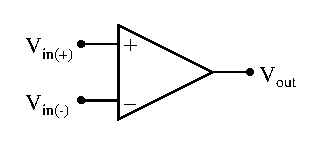
\includegraphics[width=15.5cm]{i01471x01.eps}$$

\underbar{file i01471}
%(END_QUESTION)





%(BEGIN_ANSWER)

$V_{out} = 100,000(V_{in(+)} - V_{in(-)})$

%(END_ANSWER)





%(BEGIN_NOTES)

Begrepet ``overføringsfunksjon'' er svært nyttig, og dette kan være studentenes første møte med ideen. Det er et uttrykk som brukes ofte i tekniske anvendelser, og kan betegne en ligning, en talltabell eller en graf.

I denne oppgaven er det viktig at studentene vet hvordan man utleder og bruker den grunnleggende overføringsfunksjonen for en differensialforsterker. Utfordre studentene til å uttrykke funksjonen på en mer generell form, slik at beregninger kan gjøres med andre verdier for åpen sløyfeforsterkning.

%INDEX% Electronics review: opamp as a high-gain differential amplifier

%(END_NOTES)

